\documentclass{beamer}
\usepackage{graphicx}
\usepackage{paralist}
\usepackage{outlines}

\title{DAM 110 - Weekly Overview - 16}
\author{Mendocino College - Digital Image Manipulation with Photoshop}
\titlegraphic{\vspace{-10mm}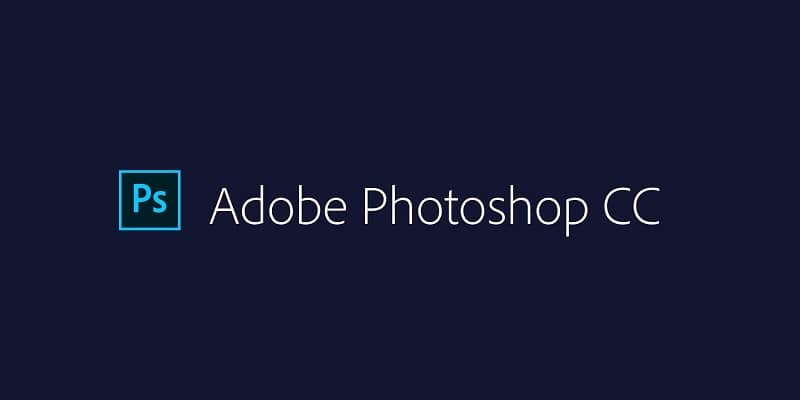
\includegraphics[width = .9\textwidth]{images/photoshop.jpg}} 
\date{\vspace{-5em}} 


\mode <presentation>
\usetheme{Warsaw}
\usecolortheme{default}

\setbeamerfont{footline}{size=\fontsize{5}{8}\selectfont}

\definecolor{darkred}{rgb}{20,0,0}
\definecolor{darkgreen}{RGB}{40,110,20}
\definecolor{darkpurple}{RGB}{30,0,30}
\definecolor{chardonnay}{RGB}{255, 255, 204}

\setbeamercolor*{palette primary}{fg=white, bg=darkgreen}


\begin{document}
	{
		\setbeamertemplate{footline}{} 
		\setbeamertemplate{headline}{} 
		\begin{frame}
			\vspace{-35pt}
			\maketitle
		\end{frame}
	}

	\section{Overview}
			\subsection{Lecture Topics}		
	\begin{frame}
		\frametitle{Lecture Topics for Week - 16}
				\begin{columns}
				\column{.5\textwidth}
				\vspace{-25pt}
				\begin{outline}
					\1 Skills
					\2 The skills which are needed to use photoshop to make money.
					\1 Professions
					\2 The jobs, careers and professions which require the use of Photoshop.
					\1 Resume
					\2 Create a Resume and Cover Letter in Photoshop.
				\end{outline}
				\column{.5\textwidth}
				\vspace{-22pt}
				\begin{center}
					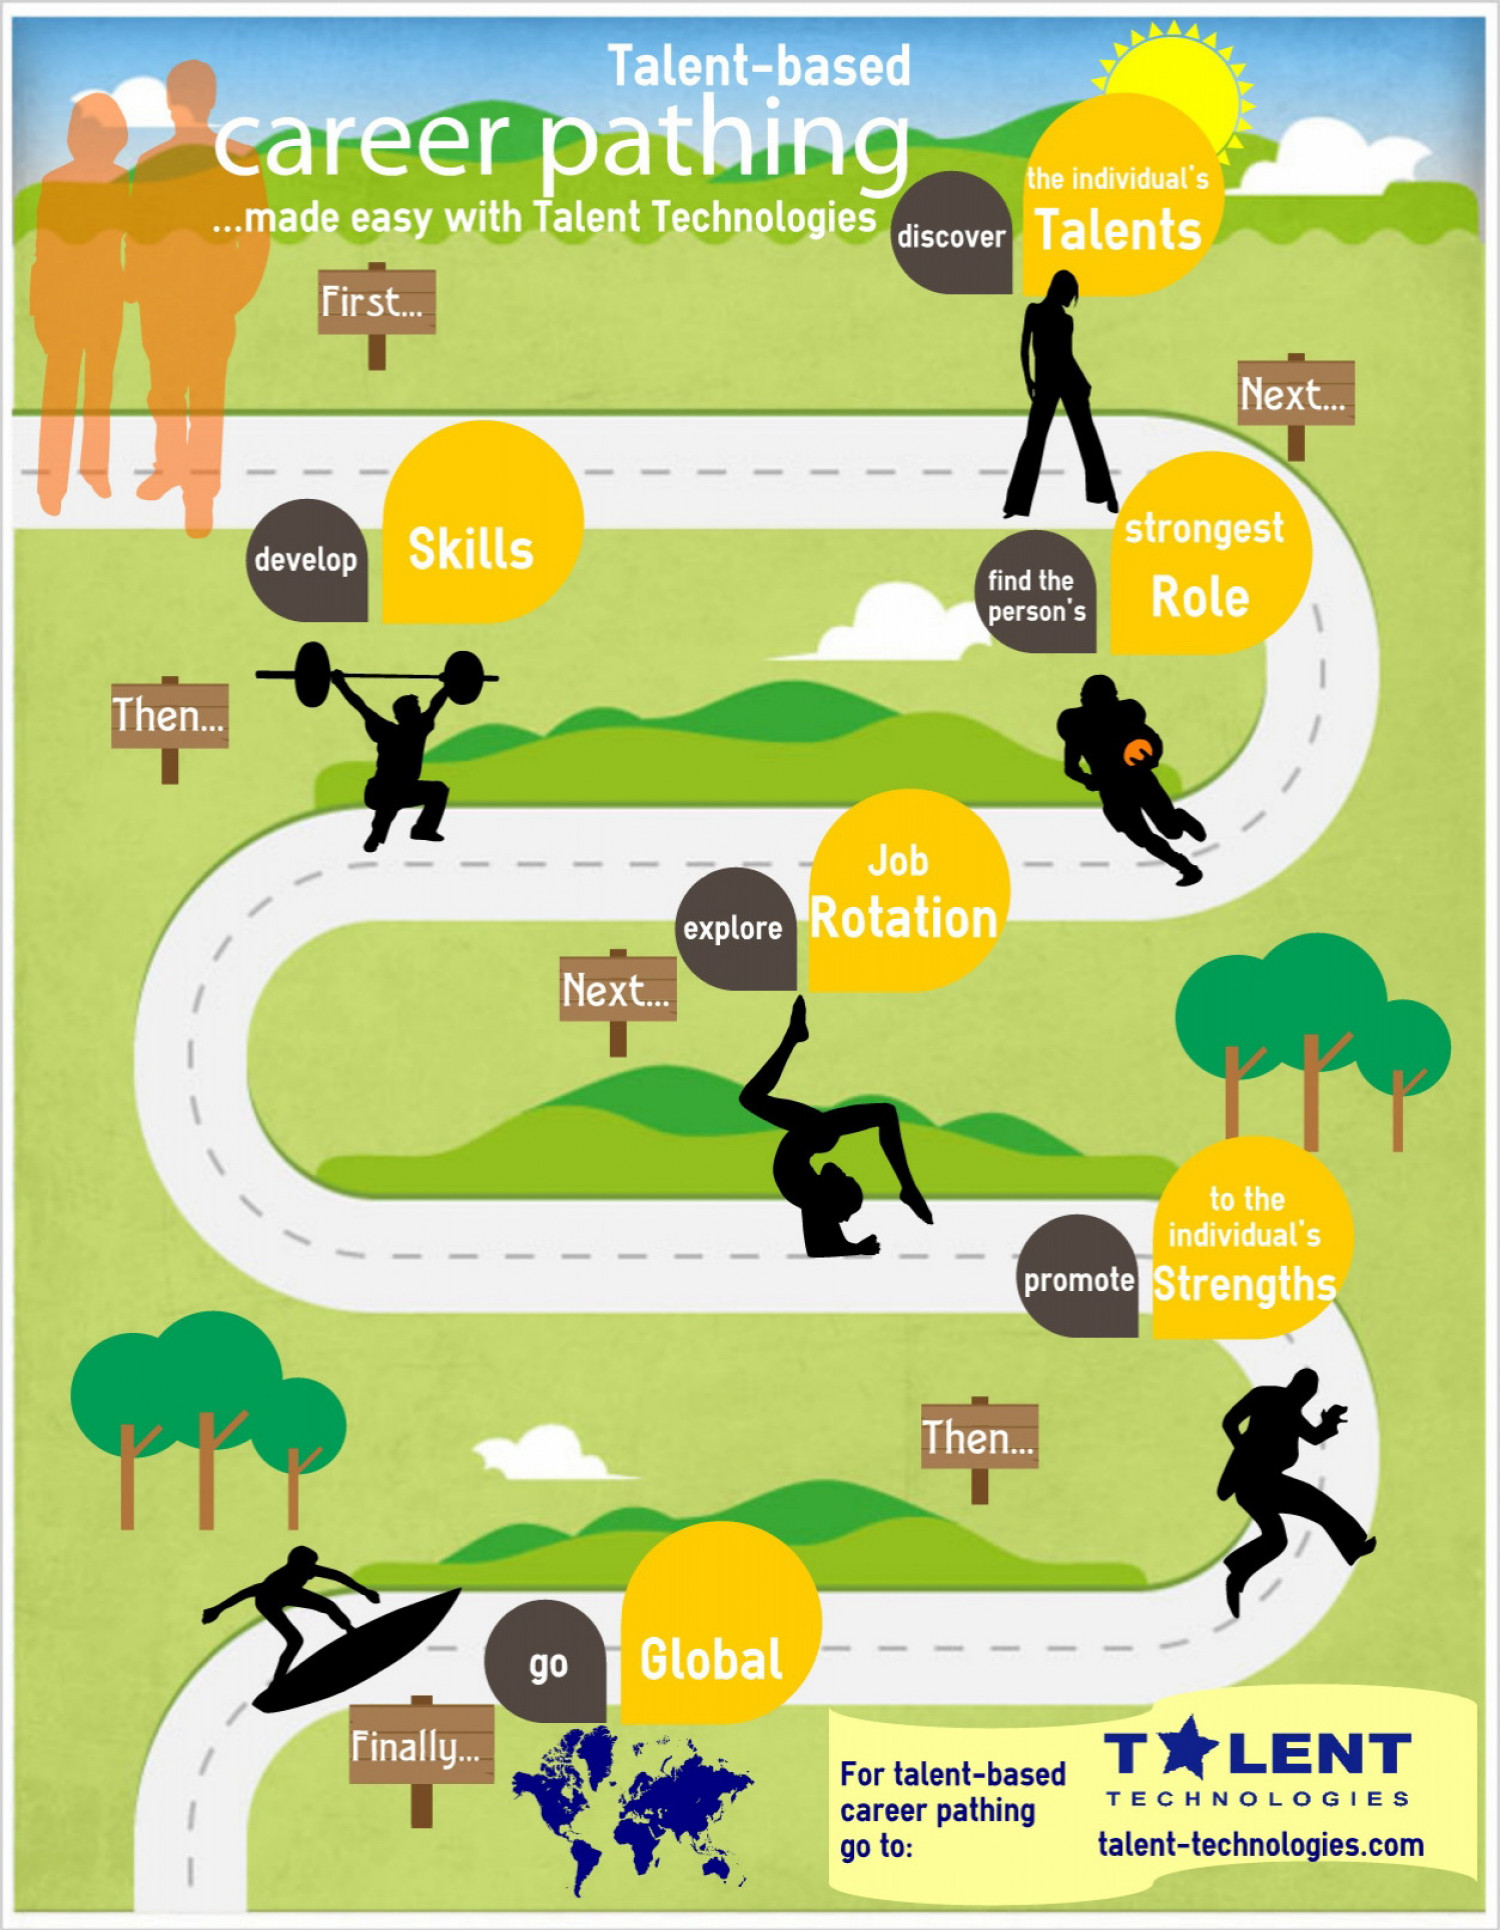
\includegraphics[width=1.10\textwidth]{images/careerpathing-infographic_51a45f3a9e17a_w1500.jpg}
				\end{center}
			\end{columns}
		\end{frame}

	\section{Lecture Topics}
			\subsection{Skills}		
				\begin{frame}
					\frametitle{Skills Needed with Photoshop}
					\begin{columns}
						\column{.5\textwidth}
						\vspace{-50pt}
						\begin{outline}
							\1 Photoshop, Illustrator, \& InDesign
							\1 Non-destructive workflow
							\1 Adding Text \& Shapes
							\1 Creating Visual Effects
							\1 Retouching and Restoration
							\1 Creativity \& Imagination
						\end{outline}
						\column{.5\textwidth}
						\vspace{-10pt}
						\begin{center}
							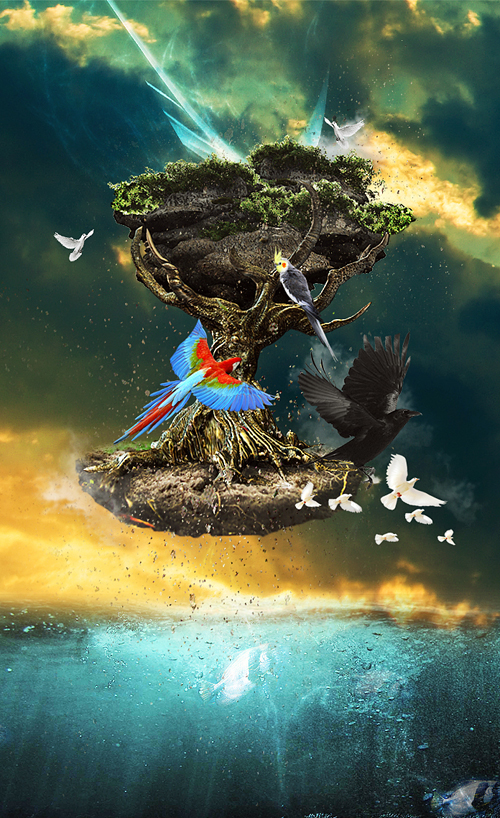
\includegraphics[width=1.0\textwidth]{images/001+Photoshop+Tutorials.jpg}
						\end{center}
					\end{columns}
				\end{frame}

			
		\subsection{Professions}		
			\begin{frame}
				\frametitle{Professions which require Photoshop}
				\begin{outline}
					\1 UI/UX
					\1 Web \& Game Development
					\1 Youtuber, Influencer, Content Creator
					\1 Advertising \& Marketing
					\1 Photography \& Videography
				\end{outline}
			\begin{center}
				\includegraphics[width=1.0\textwidth]{images/Job-Connection-Office-Worker.jpeg}
			\end{center}
			\end{frame}
		
	\subsection{Resume and Cover Letter}		
		\begin{frame}
			\frametitle{Resume and Cover Letter}
			\begin{columns}
				\column{.5\textwidth}
				\vspace{-50pt}
			\begin{outline}
				\1 Tips and Suggestions for making your own resume and cover letters.
				\1 Create your own Resume and Cover Letter in Photoshop!
			\end{outline}
								\column{.5\textwidth}
		\vspace{-10pt}
			\begin{center}
				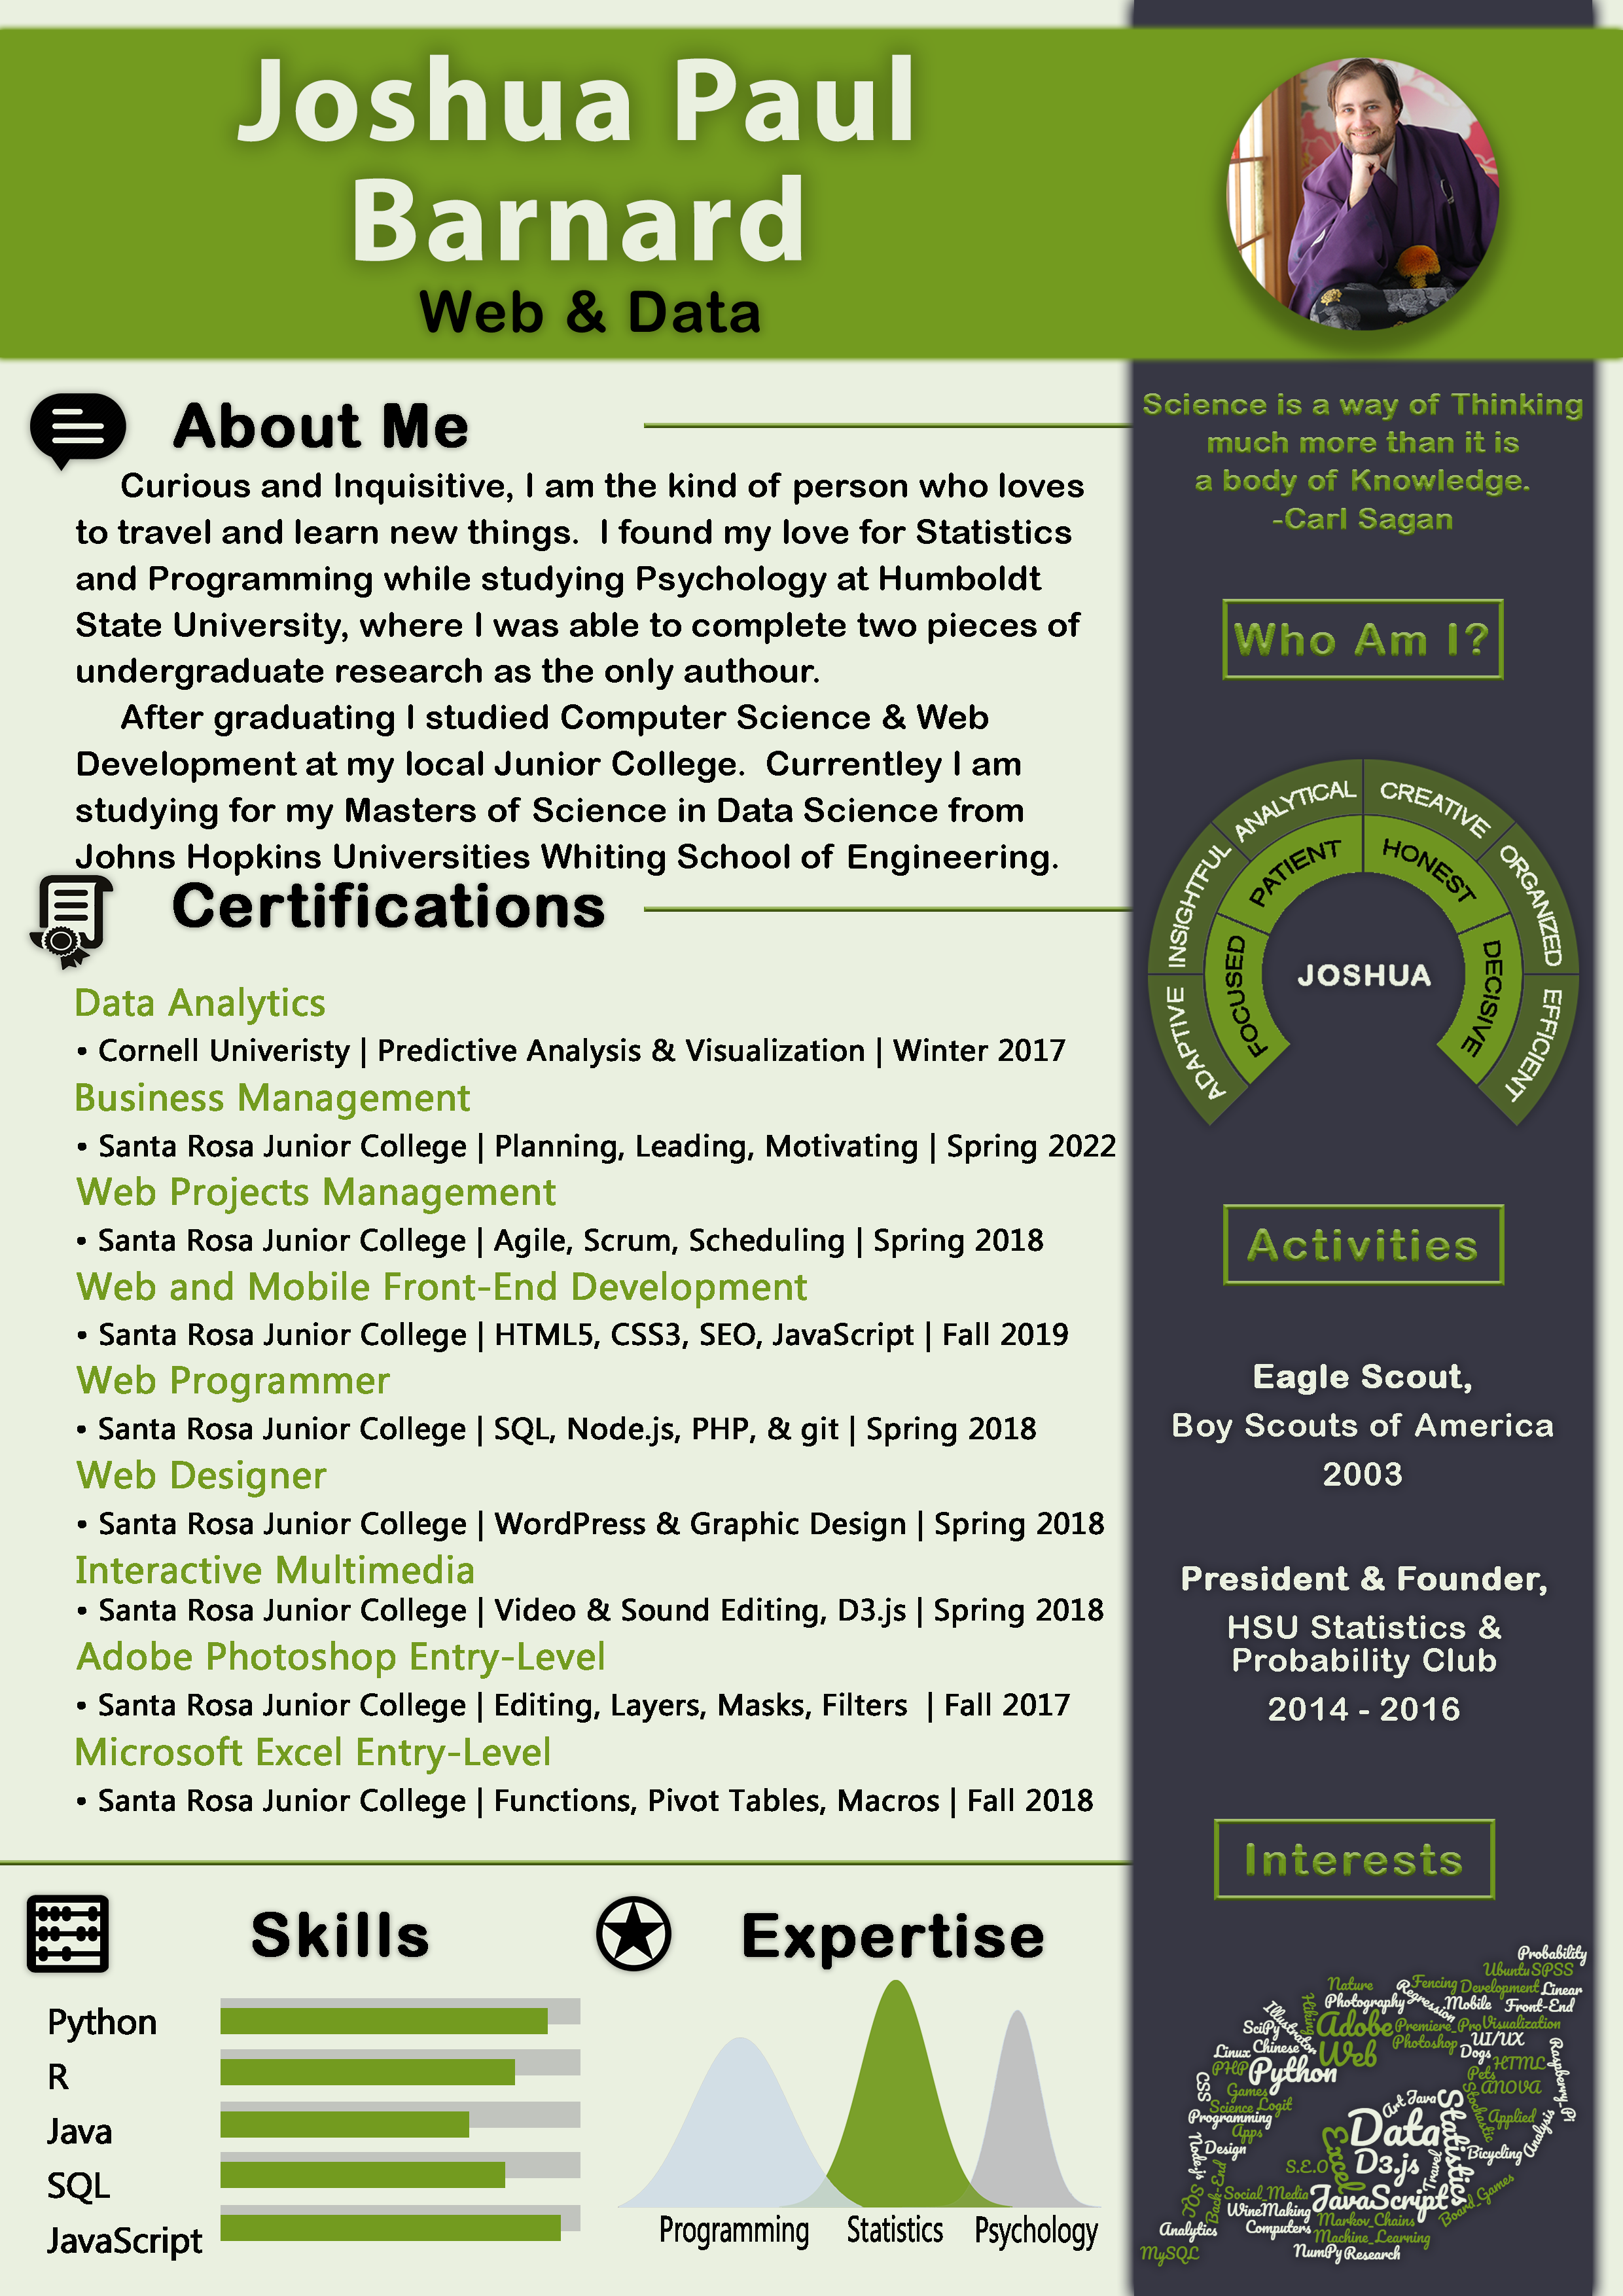
\includegraphics[width=1.0\textwidth]{images/Joshua_Paul_Barnard-second_page.png}
			\end{center}
		\end{columns}
		\end{frame}
			

\section{Exercises, Assignments and Discussion}

\subsection{Weekly Exercises}		
\begin{frame}
	\frametitle{Exercises for Week 16}
	\begin{outline}
		\1 Make a Resume, using a template:
		\2 Update the given Resume template to use when applying for work and universities.
		\1 Make a Cover Letter, using a template:
		\2 Update the given Cover Letter template to use when applying for work and school.
	\end{outline}
\end{frame}

\subsection{Discussion}		
\begin{frame}
	\frametitle{Articles/Videos for Week 16's Discussion}
	\begin{outline}
		\1 Jobs that use Photoshop
		\2  By:    MERCY UGONNA NJOKU
		\2  Pages: 8
		\2  Date:  FEB 5, 2022
		\2 https://careerkarma.com/blog/jobs-that-use-photoshop/
		\1 5 Types Of Photoshop Retouching Careers \& Positions - PRO EDU
		\2  By:  PRO EDU Photography Tutorials
		\2 https://www.youtube.com/watch?v=Pkq9MOFXusw
		\1 Photoshop as Your Career
		\2  By:  Yes I'm a Designer
		\2 https://www.youtube.com/watch?v=3rLoNKIeRUU
		\1 How To Make Money With Photoshop in 2022 (For Beginners)
		\2  By:  Mike Vestil
		\2 https://www.youtube.com/watch?v=RoWBU4zkG80
	\end{outline}
\end{frame}

\begin{frame}
	\frametitle{Research Topics}
	\begin{center}
		Research a Job Title
	\end{center}
	\begin{columns}
		\column{.5\textwidth}
		\begin{outline}
			\1 User Experience Designer
			\1 Web \& Mobile Designer
			\1 Web Developer
			\1 SEO Specialist
			\1 Digital Marketer
			\1 Advertising Copywriter
			\1 Advertising Manager
			\1 Campaign Manager
		\end{outline}
		\column{.5\textwidth}
		\begin{outline}
			\1 Graphic Designer
			\1 Animator
			\1 Content Creator
			\1 Photographer
			\1 Videographer
			\1 Art Professor
			\1 Design Architect
			\1 Design Engineer
		\end{outline}
	\end{columns}
\end{frame}
	
			
\end{document}